
\section{态射上的一大堆有限性条件}

到本节结束之时，你将会见过以下几类\trMorphism：\trQuasicompact、\trQuasiSeparated、\trAffine、有限（finite）、\trIntegral、闭（closed）、（局部）有限型（(locally) of finite type）、\trQuasifinite{}（quasifinite）——或许还有（局部）有限表现（(locally) of finite presentation）。

\textbf{8.3.1.\ 拟紧与拟分离的\trMorphism。}

概形之间的\trMorphism{} $\pi\colon X\to Y$ 称为\textbf{\trQuasicompact}的，若对 $Y$ 的每个\trAffine\trOpenSubset{} $\mathsf{U}$，$\pi^{-1}(\mathsf{U})$ 都\trQuasicompact。（等价地，任何\trQuasicompact{}开子集的原像都\trQuasicompact。这也是几何学其他分支中正确的定义。）

我们将会喜欢这个观念，理由有二：(i) 有限集比起无限集自有好处（例如，整数的有限集必有最大元；再者，关于有限的对象可以归纳地证明）；(ii) 大多数合理的概形都将是\trQuasicompact{}的。

伴随着\trQuasicompactness{}而来的，是拟分离性这个古怪的观念。称\trMorphism{} $\pi\colon X\to Y$ 是\textbf{\trQuasiSeparated}的，若对 $Y$ 的每个\trAffine\trOpenSubset{} $\mathsf{U}$，$\pi^{-1}(\mathsf{U})$ 都是一个\trQuasiSeparated{}概形（\S5.1.1）。（等价地，任何\trQuasiSeparated{}开子集的原像都\trQuasiSeparated；我们不打算操心这件事的证明。这才是能推广到几何学其他分支的那种定义。）这条假设在定理中将会很有用，而且通常与\trQuasicompactness{}连用。（因此，「\trQuasicompact{}且\trQuasiSeparated」常被缩写作「qcqs」；参看 \S5.1.2。）几类有趣的\trMorphism（源为局部\trNoetherian、\trAffine、\trSeparated——分别参看\cref{ex:quasicompact-quasiseparated-source}(b)、练习~8.3.D 与\mbox{练习~11.2.D}）都是\trQuasiSeparated{}的，而有了「\trQuasiSeparated」一词，我们陈述定理时便能更加简练。\emph{重要注记：}我们将在 \S11.1.4（「拟分离＝拟紧对角」）中给出拟分离性的一个等价定义，它用起来会简单得多。

\textbf{8.3.A.（容易的练习）}\quad 证明：两个\trQuasicompact{}\trMorphism{}的\trComposition{}仍\trQuasicompact。（两个\trQuasiSeparated{}\trMorphism{}的\trComposition{}仍\trQuasiSeparated，这也成立——但不容易。你尽可以直接证明它，但无论如何，等我们对它有了更精巧的理解之后，它会轻易地随之而来；见 \S11.1.5。）

循着\trGrothendieck{}「重要的观念是\trMorphism{}的性质而非\trObject{}的性质」的哲学（\S8.0.1），我们可以把「\trQuasicompact 的（相应地，\trQuasiSeparated 的）概形」的定义重述为「在\trScheme{}的\trCategory{}中，它在\trFinalObject{} $\Spec\mathbb{Z}$ 之上\trQuasicompact（相应地，\trQuasiSeparated）的概形」（练习~7.3.J）。

\vkexsync{B}
\begin{exercise}[容易的练习]\label{ex:quasicompact-quasiseparated-source}
\begin{enumerate}[label=(\alph*)]
\item 证明：从\trNoetherian{}概形出发的任何\trMorphism{}都\trQuasicompact。
\item 证明：从\trQuasiSeparated{}概形出发的任何\trMorphism{}都\trQuasiSeparated。于是，由练习~5.3.A，从局部\trNoetherian{}概形出发的任何\trMorphism{}都\trQuasiSeparated。这样，只与局部\trNoetherian{}概形打交道的读者，尽可以把拟分离性当作一条\trStandingHypothesis{}（standing hypothesis）。
\end{enumerate}
\end{exercise}

\textbf{8.3.2.}\ \emph{\trhCaveat{}。}\quad \cref{ex:quasicompact-quasiseparated-source}的两部分或许会让你疑心：凡源与靶皆\trQuasicompact{}的\trMorphism{} $\pi\colon X\to Y$ 都必然\trQuasicompact。这是错的；你可以核验下面这个反例。设 $Z$ 是练习~5.1.K 中构造的那个非拟分离概形，并如练习~5.1.K 那样取 $X=\Spec k[x_1,x_2,\dots]$。那个显然的\trOpenEmbedding{} $\pi\colon X\to Z$（把 $X$ 认作粘出 $Z$ 的两块之一）不\trQuasicompact。（但等你见到\trCancellationTheorem{}~11.1.1 之后，立刻就会看出：从\trQuasicompact{}的源到一个\emph{\trQuasiSeparated}的靶的任何\trMorphism{}都必然\trQuasicompact。）

\vkexsync{C}
\begin{exercise}\label{ex:quasicompact-quasiseparated-affine-local}
（对两部分都显而易见的提示：\trAffineCommunicationLemma{}~5.3.2。）
\begin{enumerate}[label=(\alph*)]
\item （\trQuasicompactness{}是对目标仿射局部的。）证明：若存在由诸\trAffine\trOpenSet{} $\mathsf{U}_i$ 构成的 $Y$ 的一个\trCover{}，使得每个 $\pi^{-1}(\mathsf{U}_i)$ 都\trQuasicompact，则\trMorphism{} $\pi\colon X\to Y$ 是\trQuasicompact{}的。
\item （拟分离性是对目标仿射局部的。）证明：若存在由诸\trAffine\trOpenSet{} $\mathsf{U}_i$ 构成的 $Y$ 的一个\trCover{}，使得每个 $\pi^{-1}(\mathsf{U}_i)$ 都\trQuasiSeparated，则\trMorphism{} $\pi\colon X\to Y$ 是\trQuasiSeparated{}的。
\end{enumerate}
\end{exercise}

\textbf{8.3.3.\ \trAffine\trMorphism。}

称概形之间的\trMorphism{} $\pi\colon X\to Y$ 是\textbf{\trAffine}的，若对 $Y$ 的每个\trAffine\trOpenSet{} $\mathsf{U}$，$\pi^{-1}(\mathsf{U})$（解读为 $X$ 的一个\trOpenSubscheme）都是\trAffineScheme。平凡地，两个\trAffine{}\trMorphism{}的\trComposition{}仍\trAffine。

\textbf{8.3.D.（快速练习）}\quad 证明：\trAffine{}\trMorphism{}既\trQuasicompact{}又\trQuasiSeparated。（后者的提示：练习~5.1.G。）

\textbf{8.3.4.\ \trhProposition{}（一个\trMorphism{}的「仿射性」这一性质是对目标仿射局部的）。}\ ——\ \emph{设 $\pi\colon X\to Y$ 是一个\trMorphism。若存在 $Y$ 的一个由\trAffine\trOpenSet{} $\mathsf{U}$ 构成的\trCover{}，使得每个 $\pi^{-1}(\mathsf{U})$ 都\trAffine，则 $\pi$ 是\trAffine{}的。}

\emph{证明。}\ 我们把\trAffineCommunicationLemma{}~5.3.2 施于「$\pi$ 在其上是仿射的」这条条件。逐条核验我们的两条判据。第一，设 $\pi\colon X\to Y$ 在 $\Spec B$ 上仿射，即 $\pi^{-1}(\Spec B)=\Spec A$。则对任意 $s\in B$，$\pi^{-1}(\Spec B_s)=\Spec A_{\pi^\sharp s}$。（你可看出这是为什么吗？）

第二，设给了 $\pi\colon X\to\Spec B$ 与 $(s_1,\dots,s_n)=B$，诸 $X_{\pi^\sharp s_i}$ 都仿射（比如说为 $\Spec A_i$）。（回想定义~6.2.8：$X_{\pi^\sharp s_i}$ 是 $X$ 中 $\pi^\sharp s_i$ 不消失的开子集。）我们希望证明 $X$ 也是仿射的。令 $A=\Gamma(X,\OO_X)$。于是 $X\to\Spec B$ 可经由\trTautologicalMap{}（tautological map）$\alpha\colon X\to\Spec A$ 分解（它由那个（同构）映射 $A\to\Gamma(X,\OO_X)$ 产生，练习~7.3.G）。
\[
\begin{tikzcd}[row sep=3.2em, column sep=5.5em]
\bigcup_i X_{\pi^\sharp s_i}=X \ar[dr, "\pi"'] \ar[rr, "\alpha"] & & \Spec A \ar[dl, "\beta"] \\
& \bigcup_i D(s_i)=\Spec B &
\end{tikzcd}
\]
我们想证明 $\alpha$ 是一个\trIsomorphism。现在，$\beta^{-1}(D(s_i))=D(\beta^\sharp s_i)\cong\Spec A_{\beta^\sharp s_i}$（\trDistinguishedOpen{}的原像还是\trDistinguishedOpen），而 $\pi^{-1}(D(s_i))=\Spec A_i$。此外，由这些观念的仿射局部性（\cref{ex:quasicompact-quasiseparated-affine-local}），$X$ 既\trQuasicompact{}又\trQuasiSeparated，于是 Qcqs 引理~6.2.9 的诸假设得到满足。故由 Qcqs 引理~6.2.9，我们有诱导出的\trIsomorphism
\[
A_{\beta^\sharp s_i}=\Gamma(X,\OO_X)_{\beta^\sharp s_i}\cong\Gamma(X_{\beta^\sharp s_i},\OO_X)=A_i.
\]
于是 $\alpha$ 诱导\trIsomorphism{} $\Spec A_i\tilde{\longrightarrow}\Spec A_{\beta^\sharp s_i}$（环的\trIsomorphism{}诱导\trAffineScheme{}的\trIsomorphism，\cref{ex:scheme-isos-ring-isos}）。于是 $\alpha$ 在覆盖 $\Spec A$ 的所有 $\Spec A_{\beta^\sharp s_i}$ 上都是\trIsomorphism，从而 $\alpha$ 是\trIsomorphism。所以 $X\to\Spec A$ 是\trIsomorphism，即 $X$ 如愿地是\trAffine{}的。\hfill$\square$

\trAffine{}\trMorphism{}的仿射局部性（命题~8.3.4）有一些并不显然的推论，见下一道练习。

\textbf{8.3.E.（有用练习）}\quad 设 $Z$ 是\trAffineScheme{} $\Spec A$ 的一个由单个方程局部切出的\trClosedSubset。（换言之：$\Spec A$ 可以被一些更小的\trOpenSet{}覆盖，而在每个这样的\trOpenSet{}上，$Z$ 都由单个方程切出。）证明：$Z$ 的补集 $Y$ 是\trAffine{}的。（若 $Z$ 整体地由单个方程 $f$ 切出，哪怕只是在集合论的层面上，这件事也是清楚的；此时 $Y=\Spec A_f$。然而 $Z$ 并不总是这种形式；见 \S19.11.10。）

\textbf{8.3.5.\ 有限与\trIntegral{}的\trMorphism。}

在定义\trFinite{}与\trIntegral{}的\trMorphism{}之前，先给出一个值得放在心里的例子。若 $L/K$ 是一个\trFieldExtension，则 $\Spec L\to\Spec K$：(i) 总是\trAffine；(ii) 当 $L/K$ \trAlgebraic{}时是\trIntegral{}的；(iii) 当 $L/K$ 有限时是\trFinite{}的。

回想：若有\trRingMorphism{} $B\to A$ 使得 $A$ 是一个\trFinitelyGenerated{}的 $B$-\trModule，则我们称 $A$ 是一个\textbf{有限}（finite）$B$-\trAlgebra。这比「$A$ 是一个\trFinitelyGenerated{}的 $B$-\trAlgebra」要强。（「有限 $B$-代数」与「有限生成 $B$-代数」这两套术语如此相像，实在不幸。）称一个\trMorphism{} $\pi\colon X\to Y$ 是\textbf{有限}的，若对 $Y$ 的每个\trAffine\trOpenSet{} $\Spec B$，$\pi^{-1}(\Spec B)$ 都是一个有限 $B$-代数的谱。据定义，有限\trMorphism{}都是\trAffine{}的。

\textbf{8.3.F.（练习：\trFinite{}性这一性质是对目标仿射局部的）}\quad 证明：若存在由诸\trAffine\trOpenSet{} $\Spec A$ 构成的 $Y$ 的一个\trCover{}，使得每个 $\pi^{-1}(\Spec A)$ 都是某个\trFinite{} $A$-代数的谱，则\trMorphism{} $\pi\colon X\to Y$ 是\trFinite{}的。

下面四个例子会让你对有限\trMorphism{}找到一些感觉。在每个例子中，你都会注意到两件事。各种情形下，这些映射作为集合的映射总是\trFiniteToOne{}（finite-to-one）的；这一点我们将在练习~8.3.J 中一般地予以验证。
你还会注意到，这些\trMorphism{}作为\trTopologicalSpace{}的映射都是\textbf{闭}（closed）的，也就是说，\trClosedSet{}的像是\trClosedSet。
我们将在练习~8.3.L 中证明有限\trMorphism{}总是闭的（并在 \S9.3.5 中给出第二个证明）。直观上，你应当把「有限」想成「闭加上\trFiber{}有限」，尽管这并不全真。我们将在\mbox{定理~28.5.2}中把这话说精确。

\emph{例~1：\trBranchedCover{}（branched covers）。}\quad 考虑由 $u\mapsto p(t)$ 给出的\trMorphism{} $\Spec k[t]\to\Spec k[u]$，其中 $p(t)\in k[t]$ 是一个次数 $n$ 的多项式（见图~\ref{fig:branched-cover}）。
这是\trFinite{}的：$k[t]$ 作为 $k[u]$-\trModule{}由 $1$、$t$、$t^2$、……、$t^{n-1}$ 生成。

\begin{figure}[htbp]
\centering
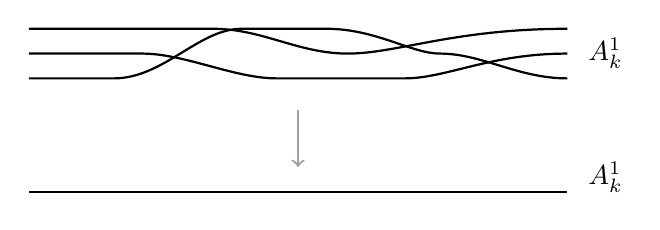
\begin{tikzpicture}[scale=0.9,line width=0.8pt]
  \draw (0,1.50) -- (2.6,1.50) .. controls (3.3,1.50) and (3.8,1.15) .. (4.5,1.15)
        .. controls (5.2,1.15) and (6.0,1.50) .. (7.6,1.50);
  \draw (0,1.15) -- (1.6,1.15) .. controls (2.2,1.15) and (2.9,0.80) .. (3.5,0.80)
        -- (5.3,0.80) .. controls (5.9,0.80) and (6.5,1.15) .. (7.6,1.15);
  \draw (0,0.80) -- (1.2,0.80) .. controls (1.9,0.80) and (2.4,1.50) .. (3.0,1.50)
        -- (4.2,1.50) .. controls (4.9,1.50) and (5.4,1.15) .. (5.8,1.15)
        .. controls (6.4,1.15) and (6.9,0.80) .. (7.6,0.80);
  \node[anchor=west] at (7.75,1.15) {$\mathbb{A}^1_k$};
  \draw[gray!75,->] (3.8,0.35) -- (3.8,-0.45);
  \draw (0,-0.80) -- (7.6,-0.80);
  \node[anchor=west] at (7.75,-0.60) {$\mathbb{A}^1_k$};
\end{tikzpicture}
\caption{由 $u\mapsto p(t)$ 给出的、以「$t$-线」盖住「$u$-线」的「\trBranchedCover{}」$\mathbb{A}^1_k\to\mathbb{A}^1_k$ 是\trFinite{}的。（依原书手绘图重绘，三股交叠为示意。）}\label{fig:branched-cover}
\end{figure}

\emph{例~2：闭嵌入（将很快于 \S9.1.1 中定义）。}\quad 设 $I$ 是\trRing{} $A$ 的一个\trIdeal，考虑由显然的映射 $A\to A/I$ 给出的\trMorphism{} $\Spec A/I\to\Spec A$（一个例子见图~\ref{fig:closed-embedding-spec-k}，取 $A=k[t]$，$I=(t)$）。这是一个\trFinite{}\trMorphism（$A/I$ 作为 $A$-\trModule{}由元素 $1\in A/I$ 生成）。

\begin{figure}[htbp]
\centering
\begin{tikzpicture}[scale=0.9,line width=0.8pt]
  \fill (0,1.70) circle (1.6pt);
  \draw[gray!75,->] (0,1.30) -- (0,0.35);
  \draw (-1.6,0) -- (1.6,0);
  \node at (0,-0.50) {$0$};
\end{tikzpicture}
\caption{由 $t\mapsto 0$ 给出的「闭嵌入」$\Spec k\to\Spec k[t]$ 是\trFinite{}的。（依原书手绘图重绘。）}\label{fig:closed-embedding-spec-k}
\end{figure}

\emph{例~3：正规化（将于 \S10.7 中定义）。}\quad 考虑\trMorphism{} $\Spec k[t]\to\Spec k[x,y]/(y^2-x^2-x^3)$，它对应于由 $x\mapsto t^2-1$、$y\mapsto t^3-t$ 给出的\trRingMorphism{} $k[x,y]/(y^2-x^2-x^3)\to k[t]$（请核验这是一个\trWellDefined{}的\trRingMorphism！）；见图~\ref{fig:normalization-nodal-cubic}。这是一个\trFinite{}\trMorphism，因为 $k[t]$ 作为 $\bigl(k[x,y]/(y^2-x^2-x^3)\bigr)$-\trModule{}由 $1$ 与 $t$ 生成。（图暗示：在靶的「\trNode{}」（node）之外，这是一个\trIsomorphism。
你可以核验这一点，办法是检验它在源中的 $D(t^2-1)$ 与靶中的 $D(x)$ 之间诱导了一个\trIsomorphism。我们还会一再地遇到这个例子！）

\begin{figure}[htbp]
\centering
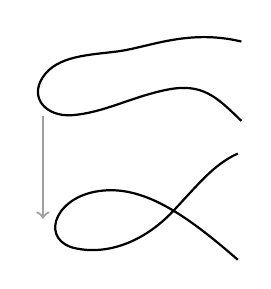
\begin{tikzpicture}[scale=0.9,line width=0.8pt]
  \draw (2.45,3.10) .. controls (1.70,3.28) and (1.15,3.02) .. (0.70,2.96)
        .. controls (0.30,2.91) and (-0.15,2.90) .. (-0.35,2.60)
        .. controls (-0.55,2.30) and (-0.30,2.04) .. (0.05,2.06)
        .. controls (0.50,2.09) and (0.90,2.32) .. (1.40,2.42)
        .. controls (1.90,2.52) and (2.10,2.32) .. (2.45,1.98);
  \draw[gray!75,->] (-0.35,2.05) -- (-0.35,0.60);
  \draw (2.40,0.02) .. controls (1.60,0.72) and (1.00,1.10) .. (0.38,0.98)
        .. controls (-0.22,0.86) and (-0.38,0.28) .. (0.12,0.18)
        .. controls (0.62,0.08) and (1.12,0.32) .. (1.48,0.70)
        .. controls (1.84,1.08) and (2.05,1.36) .. (2.40,1.52);
\end{tikzpicture}
\caption{\trNode{}三次曲线的「正规化」$\Spec k[t]\to\Spec k[x,y]/(y^2-x^2-x^3)$，由 $(x,y)\mapsto(t^2-1,\,t^3-t)$ 给出，是\trFinite{}的。（依原书手绘图重绘。）}\label{fig:normalization-nodal-cubic}
\end{figure}

\textbf{8.3.G.（重要练习：例~4，到 $\Spec k$ 的有限\trMorphism）}\quad 证明：若 $X\to\Spec k$ 是一个\trFinite{}\trMorphism，则 $X$ 是带\trDiscreteTopology{}的有限多个点的并，每个点的\trResidueField{}都是 $k$ 的一个\trFiniteFieldExtension；见图~\ref{fig:finite-morphism-spec-k}。（一个例子是 $\Spec\bigl(\mathbb{F}_8\times\mathbb{F}_4[x,y]/(x^2,y^4)\times\mathbb{F}_4[t]/(t^9)\times\mathbb{F}_2\bigr)\to\Spec\mathbb{F}_2$。）\emph{切莫}只引用某个花哨的定理了事！一条可能的进路：由\cref{ex:finite-algebra-domain-field}，任何是\trFinite{} $k$-代数的\trIntegralDomain{}必是\trField。设 $X=\Spec A$，证明 $A$ 的每个\trPrimeIdeal{} $\mathfrak{p}$ 都是\trMaximalIdeal。证明 $\Spec A$ 的诸\trIrreducibleComponent{}都是\trClosedPoint。证明 $\Spec A$ 是\trFinite{}的，进而是离散的。证明 $A$ 的诸\trResidueField{} $A/\mathfrak{m}$ 都是 $k$ 的\trFiniteFieldExtension。（向\trQuasifinite{}\trMorphism{}的推广见\mbox{练习~8.4.D}。）

\begin{figure}[htbp]
\centering
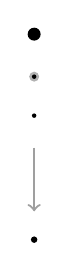
\begin{tikzpicture}[scale=0.9,line width=0.8pt]
  \fill (0,3.20) circle (2.6pt);
  \fill[gray!60] (0,2.60) circle (2.0pt);
  \fill (0,2.60) circle (0.9pt);
  \fill (0,2.05) circle (0.9pt);
  \draw[gray!75,->] (0,1.60) -- (0,0.70);
  \fill (0,0.30) circle (1.3pt);
\end{tikzpicture}
\caption{到 $\Spec k$ 的一个\trFinite{}\trMorphism{}的一幅图。更大的域被画成更大的点。（依原书手绘图重绘。）}\label{fig:finite-morphism-spec-k}
\end{figure}

\textbf{8.3.H.（容易的练习；参看\cref{ex:integrality-composition}）}\quad 证明：两个有限\trMorphism{}的\trComposition{}也有限。

\textbf{8.3.I.（练习：「到 $\Spec A$ 的有限\trMorphism{}是\trProjective{}的」）}\quad 设 $R$ 是一个 $A$-\trAlgebra。定义一个\trGradedRing{} $S_\bullet$ 如下：$S_0=A$，而对 $n>0$，$S_n=R$。（乘法结构是什么？提示：你知道如何把 $R$ 的元素彼此相乘，也知道如何把 $A$ 的元素与 $R$ 的元素相乘。）请描述一个\trIsomorphism{} $\Proj S_\bullet\tilde{\longrightarrow}\Spec R$。证明：若 $R$ 是一个\emph{有限} $A$-代数（即作为 $A$-\trModule{}\trFinitelyGenerated），则 $S_\bullet$ 是 $A$ 上\trFinitelyGenerated{}的\trGradedRing，从而 $\Spec R$ 是一个\trProjective{}的 $A$-\trScheme（\S4.5.10）。

于是有限\trMorphism{}既\trAffine（据定义）又\trProjective。逆命题也成立；见\mbox{推论~18.1.5}。

\textbf{8.3.J.（重要练习）}\quad 证明：有限\trMorphism{}有有限的\trFiber。（这是一道有用的练习，因为你终归得弄清楚怎样才能摸到一个\trMorphism{}的\trFiber{}里的点：给定 $\pi\colon X\to Y$ 与 $q\in Y$，$\pi^{-1}(q)$ 的点是什么？等我们在 \S10.3.2 中更细致地讨论过\trFiber{}之后，做起来会更容易——见注记~10.3.5——但现在就做会富于启发。）提示：设 $X=\Spec A$ 与 $Y=\Spec B$ 都是\trAffine{}的，而 $q=[\mathfrak{q}]$，那么对 $\mathfrak{q}$ 取商，便可把 $B$ 中位于 $\mathfrak{q}$ 之外的一切丢掉；证明原像是 $\Spec(A/\pi^\sharp\mathfrak{q}A)$。于是你便化归到了 $Y$ 是\trIntegralDomain{} $B$ 的谱、而 $[\mathfrak{q}]=[(0)]$ 为\trGenericPoint{}的情形。对 $(0)$ 作\trLocalization，便可把 $B$ 的其余诸点统统丢掉。证明原像是 $A$ 在 $\pi^\sharp(B\smallsetminus\{0\})$ 上\trLocalization{}后的谱。证明有限性这一条件在你所做的这些构造下得到保持，从而把问题化归到练习~8.3.G。

前两道练习表明：有限\trMorphism{}是\trProjective{}的，并且有有限的\trFiber。逆命题也成立；见\mbox{定理~18.1.6}。

关于有限性，\trFiber{}有限并非全部：值得放在心里的三个例子是例~8.3.6、练习~8.3.K 与图~19.1（图~\ref{fig:normalization-nodal-cubic} 的一个变体，它展示的\trMorphism{}是\trAffine{}的、闭的、在点上一对一的、甚至是\trMonomorphism，却不有限）。

\textbf{8.3.6.}\ \emph{\trhExample{}。}\quad \trOpenEmbedding{} $\mathbb{A}^2_k\setminus\{(0,0)\}\to\mathbb{A}^2_k$ 有有限的\trFiber，却不\trAffine（因为 $\mathbb{A}^2_k-\{(0,0)\}$ 不是\trAffine{}的，\S4.4.1），从而不有限。

\textbf{8.3.K.（容易的练习）}\quad 证明：\trOpenEmbedding{} $\mathbb{A}^1_{\mathbb{C}}\setminus\{0\}\to\mathbb{A}^1_{\mathbb{C}}$ 有有限的\trFiber{}且\trAffine，但不有限。

\textbf{8.3.7.}\ \emph{\trhDefinition{}。}\quad 称概形间的\trMorphism{} $\pi\colon X\to Y$ 是\textbf{\trIntegral}的，若 $\pi$ 是\trAffine{}的，且对每个 $\Spec B\subset Y$（\trAffine\trOpenSubset），记 $\pi^{-1}(\Spec B)=\Spec A$，其所诱导的映射 $B\to A$ 是\trIntegral{}的\trRingMorphism。据\cref{ex:integrality-affine-cover}与\cref{ex:integrality-localization-quotient}以及\trAffineCommunicationLemma{}~5.3.2，这是对目标\trAffineLocal{}的一条条件。由\cref{ex:integrality-composition}，它对\trComposition{}保持。\trIntegral{}\trMorphism{}之所以有用，主要在于：由推论~8.2.2，有限\trMorphism{}都是\trIntegral{}的。注意逆命题不成立（反例即 $\Spec\overline{\mathbb{Q}}\to\Spec\mathbb{Q}$，讨论见推论~8.2.2 的陈述之后）。

\textbf{8.3.L.（练习）}\quad 证明：\trIntegral{}\trMorphism{}是闭的，即\trClosedSubset{}的像是闭的。（从而有限\trMorphism{}是闭的。第二个证明将在 \S9.3.5 中给出。）提示：化归到仿射情形。设\trRingMorphism{} $\pi^\sharp\colon B\to A$ 诱导了\trIntegral{}\trMorphism{} $\pi\colon\Spec A\to\Spec B$；设 $I\subset A$ 切出 $\Spec A$ 的一个\trClosedSet，并令 $J=(\pi^\sharp)^{-1}(I)$；注意 $B/J\subset A/I$，然后施以 Lying Over 定理~8.2.5。

\textbf{8.3.M.（不重要练习）}\quad 设 $B\to A$ 是\trIntegral{}的。证明：对任何\trRingMorphism{} $B\to C$，所诱导的映射 $C\to A\otimes_B C$ 是\trIntegral{}的。（提示：我们希望证明 $\sum_{i=1}^n a_i\otimes c_i\in A\otimes_B C$ 在 $C$ 上\trIntegral。用「有限多个 $a_i$ 各自在 $B$ 上\trIntegral」这一事实，然后再用\cref{ex:integral-elements-subalgebra}。）等我们知道了什么是「\trBaseChange」之后，这将蕴含：一个\trMorphism{}的\trIntegrality{}这一性质对\trBaseChange{}保持，见\mbox{练习~10.4.D(e)}。

\textbf{8.3.8.}\ \emph{\trIntegral{}\trMorphism{}的诸\trFiber。}\quad 与有限\trMorphism{}不同（练习~8.3.J），\trIntegral{}\trMorphism{}的\trFiber{}未必有限。（你能想出一个例子吗？）不过，等我们在 \S10.3.2 中把\trFiber{}当作\trTopologicalSpace（甚至概形）讲出个道理之后，你就可以核验（\mbox{练习~12.1.E}）：诸\trFiber{}具有「没有任何一点落在其他任何一点的闭包之中」这一性质。

\textbf{8.3.9.\ （局部）\trFiniteType{}的\trMorphism。}

称\trMorphism{} $\pi\colon X\to Y$ 是\textbf{\trLocally\trFiniteType}（locally of finite type）的，若对 $Y$ 的每个\trAffine\trOpenSet{} $\Spec B$ 与 $\pi^{-1}(\Spec B)$ 的每个\trAffine\trOpenSubset{} $\Spec A$，所诱导的\trMorphism{} $B\to A$ 把 $A$ 表成一个\trFinitelyGenerated{}的 $B$-代数。据 $B$-概形之\trFiniteType{}性的仿射局部性（\trAffineLocal，命题~5.3.3(b)），这等价于：$\pi^{-1}(\Spec B)$ 可以被一些\trAffine\trOpenSubset{} $\Spec A_i$ 覆盖，使得每个 $A_i$ 都是\trFinitelyGenerated{}的 $B$-代数。

称\trMorphism{} $\pi$ 是\textbf{\trFiniteType}（of finite type）的，若它\trLocally\trFiniteType{}且\trQuasicompact。翻译过来：对 $Y$ 的每个\trAffine\trOpenSet{} $\Spec B$，$\pi^{-1}(\Spec B)$ 可以被\emph{有限多个}\trOpenSet{} $\Spec A_i$ 覆盖，使得所诱导的\trMorphism{} $B\to A_i$ 把 $A_i$ 表成一个\trFinitelyGenerated{}的 $B$-代数。

\textbf{8.3.10.}\ \emph{语言学上的好奇。}\quad 惯常的做法是这样来命名性质的：$P$＝局部 $P$＋\trQuasicompact。两个例外是「\trRingedSpace」（\S7.3）与「\trFinitelyPresented」（\S8.3.13）。

例：「\trStructureMorphism」 $\mathbb{P}^n_A\to\Spec A$ 是\trFiniteType{}的，因为 $\mathbb{P}^n_A$ 被形如 $\Spec A[x_1,\dots,x_n]$ 的 $n+1$ 个\trOpenSet{}所覆盖。

我们早先在 \S5.3.6 中给出的「$k$ 上\trFiniteType{}的概形」（或「\trFiniteType{} $k$-概形」）的定义，如今成了这个更一般观念的特例：「概形 $X$ 在 $k$ 上\trFiniteType」这句话的意思是，我们给定了一个\trFiniteType{}的\trMorphism{} $X\to\Spec k$（即「\trStructureMorphism」）。

下面是\trFiniteType{}\trMorphism{}享有的几条性质。

\textbf{8.3.N.（练习：「\trLocally\trFiniteType」与「\trFiniteType」都是对目标仿射局部的）}\quad 证明：若存在由诸\trAffine\trOpenSet{} $\Spec B_i$ 构成的 $Y$ 的一个\trCover{}，使得每个 $\pi^{-1}(\Spec B_i)$ 在 $B_i$ 上\trLocally\trFiniteType，则\trMorphism{} $\pi\colon X\to Y$ 是\trLocally\trFiniteType{}的。于是「\trLocally\trFiniteType」与「\trFiniteType」这两个概念都是对目标仿射局部的。

\vkexsync{O}
\begin{exercise}[有限＝\trIntegral{}＋\trFiniteType]\label{ex:finite-integral-finite-type}
\begin{enumerate}[label=(\alph*)]
\item （较易）证明：有限\trMorphism{}是\trFiniteType{}的。
\item 证明：一个\trMorphism{}是\trFinite{}的，当且仅当它既是\trIntegral{}的又是\trFiniteType{}的。
\end{enumerate}
\end{exercise}

\vkexsync{P}
\begin{exercise}[不难但重要的数道练习]\label{ex:finite-type-basic-properties}
\begin{enumerate}[label=(\alph*)]
\item 证明：每个\trOpenEmbedding{}都\trLocally\trFiniteType，从而每个\trQuasicompact{}的\trOpenEmbedding{}都是\trFiniteType{}的。证明：到局部\trNoetherian{}概形中的每个\trOpenEmbedding{}都是\trFiniteType{}的。
\item 证明：两个\trLocally\trFiniteType{}\trMorphism{}的\trComposition{}仍\trLocally\trFiniteType。（于是，既然两个\trQuasicompact{}\trMorphism{}的\trComposition{}是\trQuasicompact{}的——容易的练习~8.3.A——两个\trFiniteType{}\trMorphism{}的\trComposition{}便是\trFiniteType{}的。）
\item 设 $\pi\colon X\to Y$ \trLocally\trFiniteType，而 $Y$ 局部\trNoetherian。证明：$X$ 也局部\trNoetherian。若 $\pi\colon X\to Y$ 是一个\trFiniteType{}\trMorphism{}，而 $Y$ \trNoetherian，证明：$X$ \trNoetherian。
\end{enumerate}
\end{exercise}

\textbf{8.3.Q.（练习）}\quad 设 $X$ 是 $\mathbb{F}_p$ 上的一个\trScheme。解释如何（不用\trAxiomOfChoice）定义一个\trEndomorphism{}（endomorphism）$F\colon X\to X$，使得对每个\trAffine\trOpenSubset{} $\Spec A\subset X$，$F$ 都对应于由 $f\mapsto f^p$（对一切 $f\in A$）给出的映射 $A\to A$。（\trMorphism{} $F$ 称为\textbf{绝对\trFrobenius{}态射}（absolute Frobenius morphism）。）证明：若 $X$ 在 $\mathbb{F}_p$ 上\trLocally\trFiniteType，则 $F$ 是\trFinite{}的。

\textbf{8.3.11.}\ \emph{较不重要的定义。}\quad 称\trMorphism{} $\pi\colon X\to Y$ 是\textbf{\trQuasifinite{}}（quasifinite）的，若它\trFiniteType，且对一切 $q\in Y$，$\pi^{-1}(q)$ 都是有限集。这个定义的要点在「\trFiber{}有限」这部分；「\trFiniteType」这条假设将保证这个观念「对\trFiberProduct{}保持」，见\mbox{练习~10.4.F}。

把练习~8.3.J 与\cref{ex:finite-integral-finite-type}(a) 结合起来，便知有限\trMorphism{}都是\trQuasifinite{}的。也有\trQuasifinite{}却不有限的\trMorphism{}，例如 $\mathbb{A}^2_k\setminus\{(0,0)\}\to\mathbb{A}^2_k$（例~8.3.6）。不过我们很快就会看到：到 $\Spec k$ 的\trQuasifinite{}\trMorphism{}是\trFinite{}的（\mbox{练习~8.4.D}）。一个有有限\trFiber{}却不\trQuasifinite{}的关键例子是 $\Spec\mathbb{C}(t)\to\Spec\mathbb{C}$。另一个是 $\Spec\overline{\mathbb{Q}}\to\Spec\mathbb{Q}$。（由「$\Spec\overline{\mathbb{Q}}\to\Spec\mathbb{Q}$ 不是\trFiniteType{}的」这一事实引起的有趣行为，见警告~10.1.5。）

\textbf{8.3.12.}\ \emph{如何想象\trQuasifinite{}\trMorphism。}\quad 若 $\pi\colon X\to Y$ 是局部\trNoetherian{}概形之间的一个\trFinite{}\trMorphism，则对任意\trQuasicompact{}的\trOpenSubset{} $\mathsf{U}\subset X$，所诱导的\trMorphism{} $\pi|_{\mathsf{U}}\colon\mathsf{U}\to Y$ 是\trQuasifinite{}的。事实上，\emph{每一个}合理的\trQuasifinite{}\trMorphism{}都以这种方式出现。（这句听上去简单的陈述，实则是一个深刻而重要的结果——\trZariskiMainTheorem{}（Zariski's Main Theorem）的一种形式；见\mbox{练习~28.5.F}。）
于是，设想\trQuasifinite{}性的正确方式是：一个有限映射，再去掉某些点（的一条\trClosed\trLocus）。

\textbf{8.3.13.}\ \extrahard\ \textbf{（局部）\trFinitelyPresented{}的\trMorphism。}

下面这个「\trLocally\trFiniteType」的变体，在非诺特情形很有用。

\textbf{8.3.14.}\ \emph{\trhDefinition{}。}\quad 称一个\trRing{} $A$ 是\trFinitelyPresented{}的 $B$-代数（或 $B\to A$ 是\trFinitelyPresented{}的），如果「$A$ 在 $B$ 上有有限多个生成元与有限多个关系」：
\[
A\cong B[x_1,\dots,x_n]\big/\bigl(f_1(x_1,\dots,x_n),\dots,f_r(x_1,\dots,x_n)\bigr).
\]
若 $B$ \trNoetherian，则\trFinitelyPresented{}与\trFiniteType{}是一回事（「关系有限多条」是白送的，练习~3.6.S），所以正常人根本不会在意。

\textbf{8.3.R.（练习：有限表现蕴涵总是有限表现——代数版本）}\quad 设 $A$ 为 $B[x_1,\dots,x_n]$ 对\trIdeal{} $(f_1,\dots,f_r)$ 取商所得之环（诸 $f_i\in B[x_1,\dots,x_n]$）。又设 $Y_1,\dots,Y_m$ 作为 $B$-代数生成 $A$，于是有一个\trSurjectiveMap{} $\phi\colon B[y_1,\dots,y_m]\twoheadrightarrow A$（$y_j\mapsto Y_j$）。证明：\trIdeal{} $\ker(\phi)\subset B[y_1,\dots,y_m]$ 是\trFinitelyGenerated{}的。提示：循引理~6.4.6 的证明。

\textbf{8.3.15.\ \trhLemma{}（$A$ 在 $B$ 上的\trFinitelyPresented{}是在 $A$ 中\trAffineLocal{}的性质）。}\ ——\ \emph{$B$-代数之为\trFinitelyPresented{}这一条件，满足\trAffineCommunicationLemma{}~5.3.2 的假设。}

\emph{证明。}\ （i）\trAffineCommunicationLemma{}的第一条假设，正是下面这道练习的内容。

\textbf{8.3.S.（练习）}\quad 设 $A=B[x_1,\dots,x_n]/(f_1,\dots,f_r)$，而 $g\in A$。证明：$A_g$ 是一个\trFinitelyPresented{}的 $B$-代数。（提示：它多了一个生成元、多了一条关系。）

（ii）（这段论证是我们关于有限表现的讨论中最难的部分。）设 $A$ 是一个 $B$-代数，$g_1,\dots,g_m\in A$ 满足 $(g_1,\dots,g_m)=A$，且诸 $A_{g_i}$ 在 $B$ 上\trFinitelyPresented。我们希望证明 $A$ 在 $B$ 上\trFinitelyPresented。诸 $A_{g_i}$ 在 $B$ 上\trFinitelyGenerated，于是由命题~5.3.3(b)，$A$ 在 $B$ 上\trFinitelyGenerated，设有\trSurjectiveMap{} $\phi\colon B[x_1,\dots,x_n]\twoheadrightarrow A$。我们将证明 $I:=\ker(\phi)$ 是 $B[x_1,\dots,x_n]$ 的一个\trFinitelyGenerated{}的\trIdeal。

由于 $(g_1,\dots,g_m)=A$，我们可以选取诸 $h_j\in A$，使得 $1=h_1g_1+\cdots+h_mg_m$。把诸 $h_j$ 与诸 $g_j$ 分别提升为 $B[x_1,\dots,x_n]$ 中的 $H_j$ 与 $G_j$。令 $G_0=1-H_1G_1-\cdots-H_mG_m$，则 $G_0\in I$，且 $(G_0,G_1,\dots,G_m)=1$ 于 $B[x_1,\dots,x_n]$ 中。

\textbf{8.3.T.（练习）}\quad 证明：$I_{G_j}$ 是 $B[x_1,\dots,x_n]_{G_j}=B[x_1,\dots,x_n,y_j]/(y_jG_j-1)$ 上的一个\trFinitelyGenerated{}\trModule。（$j=0$ 的情形不同，但容易——$I_{G_0}=(1)$！）提示：引理~8.3.R。

于是，由练习~6.4.A（「模的有限生成是一条仿射局部条件」），$I$ 是一个\trFinitelyGenerated{}的 $B[x_1,\dots,x_n]$-\trModule，也就是说，$I$ 是 $B[x_1,\dots,x_n]$ 的一个\trFinitelyGenerated{}的\trIdeal，此即所愿。\hfill$\square$

\textbf{8.3.16.}\ \emph{\trhDefinition{}。}\quad 称一个 $B$-\trScheme{} $X\to\Spec B$ 在 $B$ 上\textbf{\trLocally\trFinitelyPresented}（locally finitely presented），若存在一个仿射\trCover{} $X=\bigcup\Spec A_i$，使得每个 $A_i$ 都在 $B$ 上\trFinitelyPresented。由引理~8.3.15，这等价于：对 $X$ 的\emph{一切}\trAffine\trOpenSubset{} $\Spec A$，$A$ 都在 $B$ 上\trFinitelyPresented。

\textbf{8.3.U.（练习：「\trLocally\trFinitelyPresented{}\trMorphism」这一概念对目标是\trAffineLocal{}的）}\quad 设 $\pi\colon X\to Y$ 是概形间的一个\trMorphism。证明：当 $\Spec B\subset Y$ 取遍 $Y$ 的诸\trAffine\trOpenSubset{}时，「$\pi\colon\pi^{-1}(\Spec B)\to\Spec B$ 在 $\Spec B$ 上\trLocally\trFinitelyPresented」这一条件满足\trAffineCommunicationLemma{}的假设。（这比引理~8.3.15 显著容易。）

\textbf{8.3.17.}\ \emph{\trhDefinition{}。}\quad 称\trMorphism{} $\pi\colon X\to Y$ 是\textbf{\trLocally\trFinitelyPresented}（locally finitely presented；或\textbf{局部有限表现的}，locally of finite presentation）的，若对 $Y$ 的每个\trAffine\trOpenSet{} $\Spec B$，$\pi^{-1}(\Spec B)\to\Spec B$ 在 $\Spec B$ 上\trLocally\trFinitelyPresented。由练习~8.3.U，只需在 $Y$ 的单独一个仿射覆盖上检验即可。（于是这涵盖了定义~8.3.16。）

\vkexsync{V}
\begin{exercise}\label{ex:locally-finitely-presented-covers}
设 $\pi\colon X\to Y$ 是概形间的一个\trMorphism。
\begin{enumerate}[label=(\alph*)]
\item 证明：若 $\pi$ \trLocally\trFinitelyPresented，则对 $Y$ 的\emph{任意}\trOpenSubscheme{} $\Spec B$ 与 $X$ 的\emph{任意}满足 $\pi(\Spec A)\subset\Spec B$ 的\trAffine\trOpenSubscheme{} $\Spec A$，$A$ 都是一个\trFinitelyPresented{}的 $B$-代数。
\item 设 $\bigcup\Spec A_i=X$ 是 $X$ 的一个仿射开覆盖，而诸 $\Spec B_i$ 是 $Y$ 的满足 $\pi(\Spec A_i)\subset\Spec B_i$ 的\trAffine\trOpenSubset。设每个 $A_i$ 都在 $B_i$ 上\trFinitelyPresented。证明：$\pi$ \trLocally\trFinitelyPresented。
\end{enumerate}
\end{exercise}

\textbf{8.3.W.（练习）}\quad 证明：\trOpenEmbedding{}都\trLocally\trFinitelyPresented。

\textbf{8.3.X.（练习）}\quad 证明：两个\trLocally\trFinitelyPresented{}\trMorphism{}的\trComposition{}仍\trLocally\trFinitelyPresented。

\textbf{8.3.18.}\ \extrahard\ \emph{\trhRemark{}。}\quad 称\trMorphism{} $\pi\colon X\to Y$ 是\trLocally\trFinitelyPresented{}的，当且仅当：对 $Y$-概形的每个\trProjectiveSystem{}（projective system）$\{S_\lambda\}_{\lambda\in I}$（其中每个 $S_\lambda$ 都是\trAffineScheme），自然映射
\[
\colim_{\lambda}\,\Hom_Y(S_\lambda,X)\longrightarrow\Hom_Y\bigl(\underset{\lambda}{\lim}\,S_\lambda,\,X\bigr)
\]
是双射（参看 [Gr-EGA, IV$_3$, 8.14.2]）。把\trLocally\trFinitelyPresented{}\trMorphism{}刻画为「保持极限」的这一特征可能有用。

\textbf{8.3.19.}\ \emph{\trhDefinition{}。}\quad 称一个\trMorphism{}是\textbf{\trFinitelyPresented}（finitely presented；或\textbf{有限表现的}，of finite presentation）的，若它\trLocally\trFinitelyPresented、\trQuasicompact{}且\trQuasiSeparated。特别地，\trFinitelyPresented{}\trMorphism{}这一概念是对目标仿射局部的。

这条定义违反了「擦去『局部』就等于加上『拟紧且』」这条原则（注记~8.3.10）。但它的动机是好的：\trFinitelyPresented{}意味着「在一切可能的方面都有限」（每个仿射开集对应的代数有有限多个生成元、有限多个关系；这样的仿射开集有有限多个，它们盖住了全空间；而它们的交也被有限多个仿射开集盖住）——对一个并不真的诺特的概形而言，这就是你所能指望的全部了。\mbox{练习~10.3.H} 把这一点讲精确，并解释这个观念在实践中常常如何出现。

若 $Y$ 局部\trNoetherian，则\trLocally\trFinitelyPresented{}与\trLocally\trFiniteType{}是一回事，且\trFinitelyPresented{}与\trFiniteType{}是一回事。所以，如果你是个诺特型的人，就无须为这个观念操心。\footnote{译注：此处戏拟「只与诺特情形打交道的人」，与上文 8.3.14 的「正常人」相映成趣。}
